 \chapter{Analisis}
\label{chap:analysis}
Pada bab ini, akan dijelaskan mengenai analisis \textit{input} dan fitur perangkat lunak, deskripsi pengguna perangkat lunak,  pengembangan perangkat lunak, \textit{use case} dari perangkat lunak serta diagram aktifitas dari perangkat lunak.
\section{Analisis Input}
\subsection{Analisis File Excel Jadwal Mengawas Ujian}
Sub bab ini akan membahas analisis file excel yang dikeluarkan oleh TU(Tata Usaha).\\
TU FTIS mengeluarkan jadwal setiap semester yang dibagikan kepada dosen FTIS. 
berikut ini contoh file excel yang dikeluarkan oleh TU. 
\begin{figure}[H]
	\centering
	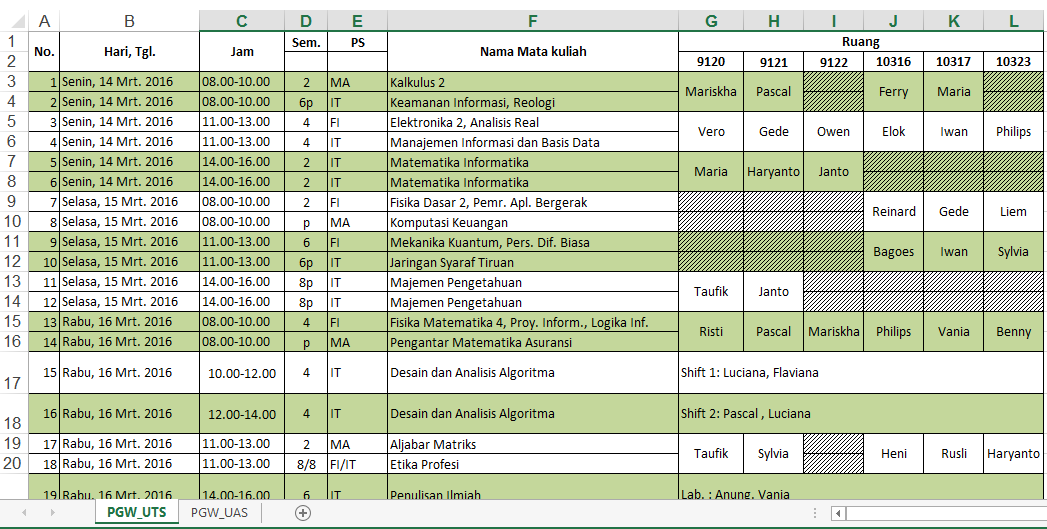
\includegraphics[scale=0.5]{Gambar/scJadwal}
	\caption{Jadwal mengawas ujian FTIS}
	\label{fig:jadwalLamapng}
	\end{figure}

Berikut penjelasan kolom-kolom yang ada di gambar \ref{fig:jadwalLamapng}.\\
File excel jadwal mengawas ujian yang dipublikasikan Tata Usaha FTIS yang terdiri dari 12 kolom A sampai dengan L. TU meentukan jumlah ruangan yang dipakai berdasarkan jumlah peserta ujian dibagi dengan jumlah dosen pengawas ujian. Setiap dosen dapat mengawas lebih dari satu matakuliah pada satu ruangan.  
Tabel ~\ref{tab:penjelasan_kolom} menjelaskan rincian dari masing-masing kolom pada excel tersebut. 
\begin{table}[H]
		\centering
		\caption{Tabel penjelasan kolom pada excel mengawas ujian}
		\label{tab:penjelasan_kolom}
\begin{tabular}{|c|p{12cm}|}
		\hline
		\textbf{No} & \textbf{Kolom dan Deskripsi} \\ \hline \hline
		1 & \textbf{No}\\
			&	Menyatakan nomer urut jadwal mengawas ujian.\\ \hline
		2 & \textbf{Hari, Tanggal}\\
			&	Kolom dalam bentuk String berisi hari dan tanggal. Terdapat singkatan yang diberikan TU dalam contoh ini  Mrt. menunjukan bulan Maret\\ \hline	
		3 & \textbf{Jam}\\
			&	Kolom ini bertipe String dan menerangkan pukul dilaksakannya mengawas ujian.\\ \hline
		4 & \textbf{Semester}\\
			&	Kolom ini bertipe String dan mengerangkan semester dari mata kuliah yang diujiankan . Terdapat simbol p yang menerangkan matakuliah pilihan\\ \hline
		5 & \textbf{PS}\\
			&	Bertipe string berisi program studi yang terkait dengan ujian mata kuliah tersebut.\\ \hline
		6 & \textbf{Nama Mata Kuliah}\\
			&	Kolom bertipe String dan berisi tentang mata kuliah yang diujiankan.\\ \hline
		7 & \textbf{Ruangan}\\
			&	Kolom dengan merge 6 kolom dan pada baris kedua terdapat 6 kolom ruangan ujian yaitu 9120, 9121, 9122, 10316, 10317, 10323. Masing kolom ruangan berisi nama pengawas ujian bertipe String. Ruangan tidak terpakai ditandai dengan garis-garis miring. Jika ada isi kolom ruangan yang dimerge sebanyak 6 kolom menandakan ruangan tersebut adalah laboratorium komputer FTIS.\\ \hline
	\end{tabular}	
\end{table}

Dari rincian tabel ~\ref{tab:penjelasan_kolom} berikut analisis \textit{flowchart} cara perangkat lunak membaca file excel : 
\begin{figure}[H]
	\centering
	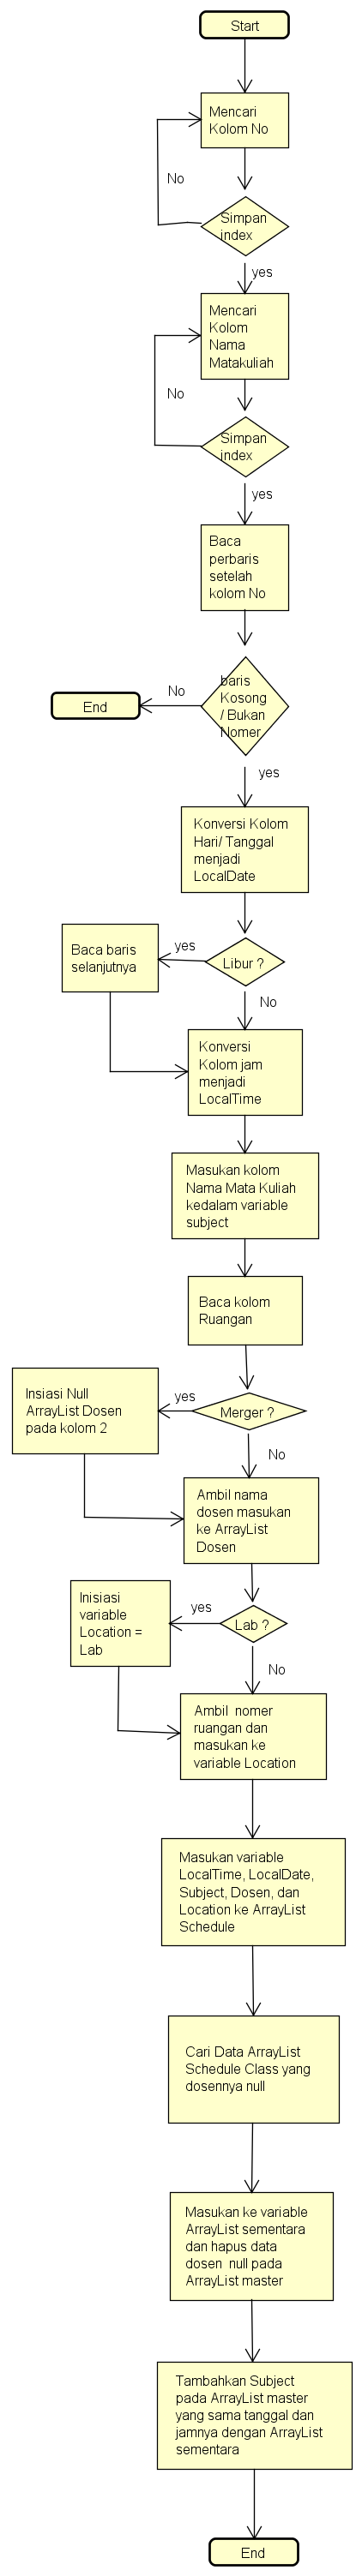
\includegraphics[scale=0.5]{Gambar/FlowchartBacaExcel}
	\caption{\textit{Flowchart} membaca excel}
	\label{fig:flowchartMembacaExcel}
	\end{figure}
\begin{enumerate}
	\item \textit{Sheet} yang dibaca merupakan \textit{Sheet} pertama.
	\item Kolom \textbf{No.} dapat dijadikan acuan dalam membaca baris jadwal Excel pada perangkat lunak. Jika PL menemukan kolom No pada excel maka simpan baris dan kolomnya pada variabel tertentu untuk menandakan bahwa baris selanjutnya merupakan data yang dibutuhkan oleh perangkat lunak. Selanjutnya nomer pada kolom No. juga dapat dijadikan penanda dalam perangkat lunak menentukan banyak data yang dibaca, jika baris selanjutnya dari kolom No. merupakan angka maka dipastikan baris tersebut memuat data jadwal mengawas.
		\item Kolom \textbf{Hari, Tgl.} memuat tanggal dan hari ujian menggunakan koma (,) sebagai pemisah hari dan tanggal dan titik (.) sebagai penanda singkatan bulan. Untuk mendapatkan tanggal yang sesuai dengan format \textit{LocalDate} maka perangkat lunak harus melakukan \textit{parsing} memisahkan hari dengan tanggal, kemudian mengkonversi bulan menjadi sebuah angka sehingga sesuai dengan format \textit{LocalDate}, lalu disimpan pada sebuah variabel.
		\item Kolom \textbf{Jam} menggunakan \textit{hyphen}(-) sebagai pemisah antara jam dimulainya ujian dan waktu ujian berakhir. perangkat lunak dapat melakukan \textit{parsing} untuk memisahkan waktu tersebut menjadi dua variabel, lalu dikonversi sesuai dengan ketentuan \textit{LocalTime}.
		\item Kolom \textbf{Nama Mata kuliah} memuat nama mata kuliah yang diujiankan, karena satu dosen dapat mengawas salah satu dari 2 matakuliah sehingga pada kolom ruangan yang memuat dua matakuliah yang ditandai dengan \textit{merger} dua baris yang berisi nama pengawas ujian.
		\item kolom \textbf{Ruangan} pada kolom ini terdapat 6 ruangan yang masing-masing kolom dan baris akan disimpan pada varible untuk dicocokan nanti pada saat membaca file excel satu per satu untuk menentukan lokasi ujian tersebut berlangsung.
		\item Jika perangkat lunak menemukan kata \textit{LIBUR} atau menemukan mata kuliah yang tidak ada dosen pengawasnya maka baris tersebut akan dilewati menuju baris selanjutnya.
		\item Jika perangkat lunak menemukan kata \textit{Shift} atau \textit{Lab} maka otomatis perangkat lunak akan menginisiasi tempat berlangsungnya ujian adalah Laboratorium Komputer.
		\item Semua variabel LocalDate, LocalTime, \textit{subject}, dosen, dan \textit{location} yang telah terisi kemudian dimasukan ke dalam sebuah ArayList \textit{schedule}.
		\item ArrayList \textit{schedule} kemudian diperiksa kembali sehingga jika pada data excel dosen memiliki 2 jadwal mengawas, maka pada ArrayList \textit{schedule} satu dosen tersebut memiliki 2 \textit{subject}.
		\item Poses ini menghasilkan \textit{output} berupa sebuah ArrayList \textit{schedule} yang memuat semua data file excel jadwal mengawas ujian yang telah dikonversi dan distandarisasi. 
\end{enumerate}

Selanjutnya adalah analisis berupa wawancara dengan dosen mengenai jadwal mengawas ujian. Hasilnya dosen FTIS tidak memerlukan kolom semseter dan program studi pada file excel jadwal mengawas. Hal ini disebabkan karena dosen FTIS dapat saling mengawas ujian antar program studi selama program studi tersebut masih dalam lingkup FTIS.Dari analisis tersebut maka kolom yang butuhkan untuk ditampilkan pada PL, yaitu :
\begin{table}[H]
		\centering
		\caption{Tabel analisa kolom pada excel mengawas ujian}
		\label{tab:analisa_kolom}
\begin{tabular}{|c|p{12cm}|}
		\hline
		\textbf{No} & \textbf{Kolom dan Deskripsi} \\ \hline \hline
		1 & \textbf{Hari, Tanggal}\\
			&	Kolom ini bertipe String dan terdapat singkatan seperti Mrt, maka akan dibuatkan fungsi pada saat implementasi agar seragam dan sesuai dengan format tgl dan waktu pada Java.\\ \hline	
		2 & \textbf{Jam}\\
			&	Kolom ini bertipe String, maka dibutuhkan konversi String kedalam fungsi jam pada saat implementasi.\\ \hline
		3 & \textbf{Nama Mata Kuliah}\\
			&	Kolom ini dapat menerangkan deskripsi mata kuliah pada PL.\\ \hline
		4 & \textbf{Dosen}\\
			&	Kolom ini merupakan isi dari tabel kelas pada excel, pada PL akan ditampilkan sebagai kolom tersendiri menerangkan nama pengawas ujian.\\ \hline		
		7 & \textbf{Ruangan}\\
			&	Kolom ini akan berisi ruangan ujian, mata kuliah, waktu dan tanggal.\\ \hline
	\end{tabular}
\end{table}

\subsection{Flowchart Konversi ArrayList Jadwal ke iCalendar}
Setelah dibaca file excel akan berubah menjadi ArrayList \textit{schedule}, kemudian data list tersebut yang menjadi \textit{input} untuk dikonversi menjadi iCalendar. Berikut alur dari konversi tersebut :

\begin{figure}[H]
	\centering
	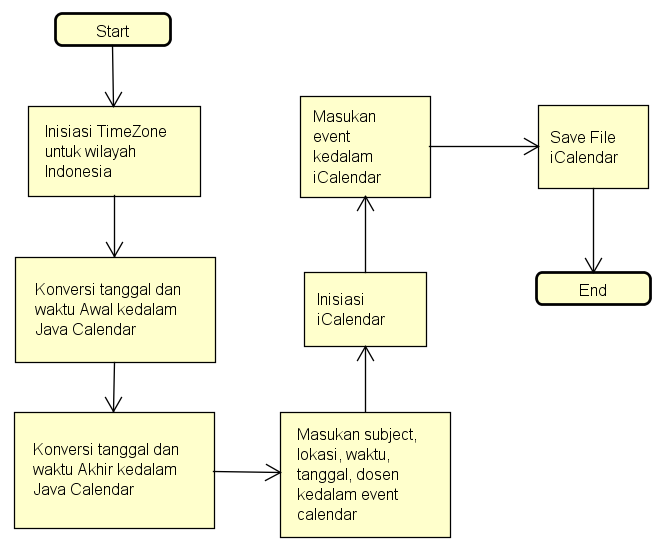
\includegraphics[scale=0.6]{Gambar/FlowchartConvertiCalendar}
	\caption{\textit{Flowchart} alur konversi excel ke iCalendar}
	\label{fig:flowchartKonversiiCalendar}
	\end{figure}
\begin{enumerate}
	\item Menginisiasi waktu indonesia.
	\item Mengkonversi waktu awal atau waktu masuk ujian kedalam format Java Calendar.
	\item Mengkonversi waktu akhir atau waktu selesai ujian kedalam format Java Calendar.
	\item Masukan mata kuliah/\textit{subject}, lokasi, jam, tanggal dari ArrayList jadwal kedalam variabel event Kalender.
	\item Inisiasi iCalendar.
	\item Masukan semua komponen event pada iCalendar.
	\item \textit{Output} icalendar dapat disimpan pada alamat folder yang diinginkan.
\end{enumerate}

\subsection{Analisis Kebutuhan Perangkat Lunak}
Perangkat Lunak ini akan memiliki fitur sebagai berikut : 
	\begin{enumerate}
		\item Perangkat lunak ini dapat menerima dan membaca\textit{input} file excel jadwal mengawas ujian yang dikeluarkan oleh TU FTIS.
		\item Perangkat lunak ini dapat mengubah file excel menjadi iCalendar.
		\item File iCalendar dapat diunduh oleh pengguna.
		\item Pengguna dapat melakukan \textit{sort} terhadap nama pengawas ujian.
	\end{enumerate}

\subsubsection{Deskripsi Pengguna}
Pengguna perangkat lunak ini merupakan dosen yang aktif mengajar di FTIS.
	
\section{Use Case Perangkat Lunak}

Berikut diagram use case berserta skenario yang tertera pada gambar \ref{fig:useCaseJadwal}

\begin{figure}[h]
	\centering
	\includegraphics[scale=0.5]{Gambar/useCaseJadwal}
	\caption{Diagram use case perangkat lunak konversi jadwal mengawas ujian}
	\label{fig:useCaseJadwal}
	\end{figure}

\begin{enumerate}
	\item Skenario Memasukan input file excel \\
	{\renewcommand\labelitemi{}
		\begin{itemize}
			\item Deskripsi		: Kegiatan memasukan input file excel.
			\item Aktor				: Pengawas
			\item Prakondisi	: -
			\item Skenario		:
				\begin{itemize}
					\item Pengawas memasukan file excel mengawas ujian.
					\item PL membaca file excel lalu menkonversi ke ArrayList jadwal.
					\item PL menampilkan jadwal dalam bentuk TableView.
				\end{itemize}
		\end{itemize}
		}
		
	\item Skenario Melakukan Sorting nama
	{\renewcommand\labelitemi{}
	\begin{itemize}
			\item Deskripsi		: Kegiatan mensorting jadwal mengawas.
			\item Aktor				: pengawas
			\item Prakondisi	: -
			\item Skenario		:
				\begin{itemize}
					\item Pengawas menuliskan nama pengawas pada kolom filter di PL.
					\item PL mengambil data nama pengawas dan mencocokannya dengan ArrayList jadwal.
					\item PL mengabil data nama pengawas yang sesuai dengan masukan Pengawas, lalu memisahkannya ke variable ArrayList sementara.
					\item PL mengatur kembali urutan tabel jadwal sesuai nama pengawas yang dimasukan Pengawas.
				\end{itemize}
		\end{itemize}
		}
		
		\item Skenario Mengunduh File iCal 
		{\renewcommand\labelitemi{}
		\begin{itemize}
			\item Deskripsi		: Kegiatan Mengunduh file iCal.
			\item Aktor				: Dosen 
			\item Prakondisi	: -
			\item Skenario		:
				\begin{itemize}
					\item Pengawas memilih jadwal yang akan dikonversi.
					\item Pengawas mengklik tombol Convert to iCal pada PL.
					\item PL mengambil item yang diseleksi oleh Pengawas.
					\item PL mengkonversi jadwal yang dipilih Pengawas.
					\item Pengawas menentukan alamat destinasi file iCalendar dan memasukan nama file iCalendar.
					\item PL akan menyimpan file iCalendar ditempat yang dipilih oleh Pengawas.
				\end{itemize}
		\end{itemize}
		}
		
\end{enumerate}

\section{Diagram Aktifitas}
Pada subbab ini akan dibahas mengenai prosedur setiap aktifitas dari perangkat lunak.

\subsection{Memasukan Excel Jadwal Mengawas Ujian}
Tahap ini merupakan tahap awal proses file input dimasukkan kedalam perangkat lunak dimana file input yang dimaksud merupakan excel jadwal yang dikeluarkan TU FTIS. Berikut step-step untuk memasukan excel kedalam perangkat lunak.
\begin{figure}[h]
	\centering
	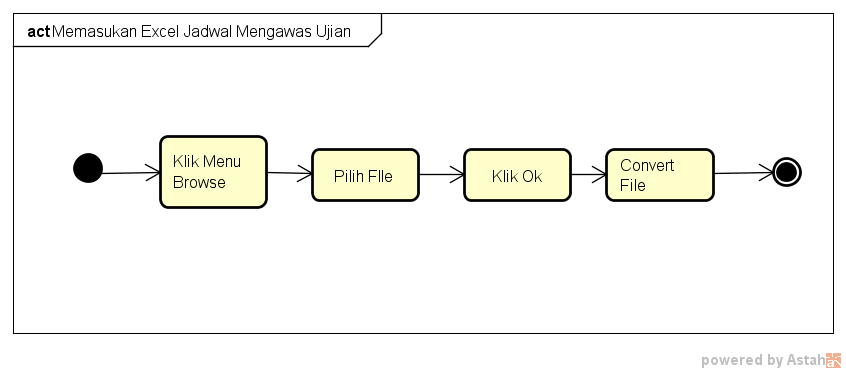
\includegraphics[scale=0.3]{Gambar/Memasukan-Excel-Jadwal-Mengawas-Ujian}
	\caption{Prosedur memasukan file excel jadwal mengawas ujian}
	\end{figure}
	
\begin{enumerate}
	\item Pengguna mengklik menu Browse yang ada di perangkat lunak. 
	\item Perangkat lunak menseleksi file yang berekstensi .xlsx yang dapat dipilih oleh pengguna.
	\item Pengguna memilih file excel yang akan dimasukkan.
	\item Pengguna mengklik tombol oke pada window.
	\item Pengguna mengklik tombol Convert untuk mengkonversi file excel.
	\item Perangkat lunak mengkonversi file excel menjadi ArrayList jadwal.
	\item Perangkat Lunak menampikan TableView jadwal yang telah dikonversi. 
\end{enumerate}

\subsection{Sorting Nama Pengawas}
Tahap ini menjelaskan bagaimana pengguna dapat memanfaatkan fitur dari perangkat lunak dengan mensorting nama dosen, dengan begitu jadwal pengawas yang dicari dapat diunduh dengan mudah. Berikut step-step untuk mensorting nama pengawas.
\begin{figure}[H]
	\centering
	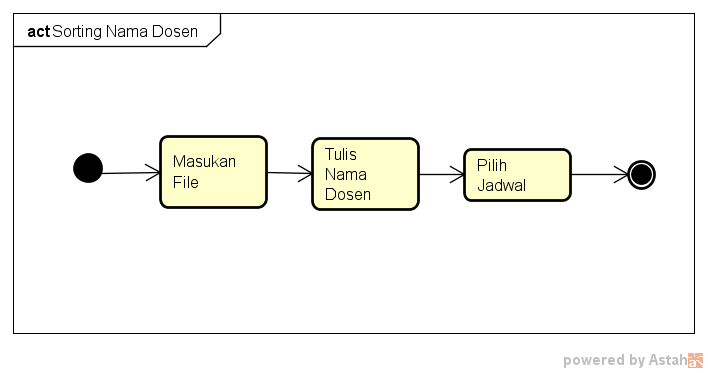
\includegraphics[scale=0.5]{Gambar/Sorting-Nama-Dosen}
	\caption{Prodsedur sorting nama pengawas}
	\end{figure}

\begin{enumerate}
	\item Pengguna menuliskan nama pengawas yang dicari.
	\item Perangkat lunak mencocokan nama pengawas dengan ArrayList jadwal.
	\item Data dengan nama pengawas yang sama akan disimpan pada ArrayList sementara.
	\item Atur kembali urutan tabel menggunakan ArrayList sementara lalu tampilkan ke pengguna.
\end{enumerate}

\subsection{Unduh File iCal}
Tahap ini merupakan tahap terakhir, file excel yang telah dimasukkan lalu dikonversi menjadi iCal selanjutnya pengguna tinggal memilih jadwal mana yang akan diunduh. File iCal yang telah dikonversi tersebut dapat diintegrasikan dengan aplikasi iCalendar seperti Google Calendar, Microsoft Outlook, dan Apple Calendar. Berikut step-step untuk mengunduh file iCal.
\begin{figure}[h]
	\centering
	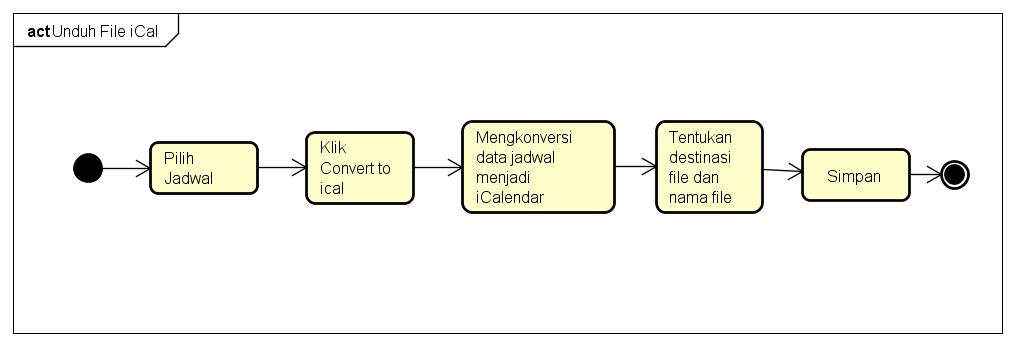
\includegraphics[scale=0.5]{Gambar/Unduh-File-iCal}
	\caption{Prosedur Mengunduh File iCal}
	\end{figure}

\begin{enumerate}
	\item Pengguna memilih jadwal yang akan dikonversi pada tabel.
	\item Pengguna mengklik tombol Convert to iCal pada perangkat lunak.
	\item Perangkat lunak mengkonversi jadwal yang dipilih oleh pengguna menjadi iCalendar.
	\item Pengguna menentukan destinasi folder penyimpanan dan menuliskan nama file iCalendar.
	\item Pengguna mengklik tombol simpan pada perangkat lunak.
\end{enumerate}

\section{Pemodelan Kelas}
Setelah file excel mengawas ujian tersebut dijabarkan dan dianalisis, pada subbab ini akan di jelaskan mengenai pembagian fungsi
kelas dalam rancangan perangkat lunak.

\subsubsection{Pemodelan Rancangan Kelas}
\begin{figure}[H]
	\centering
	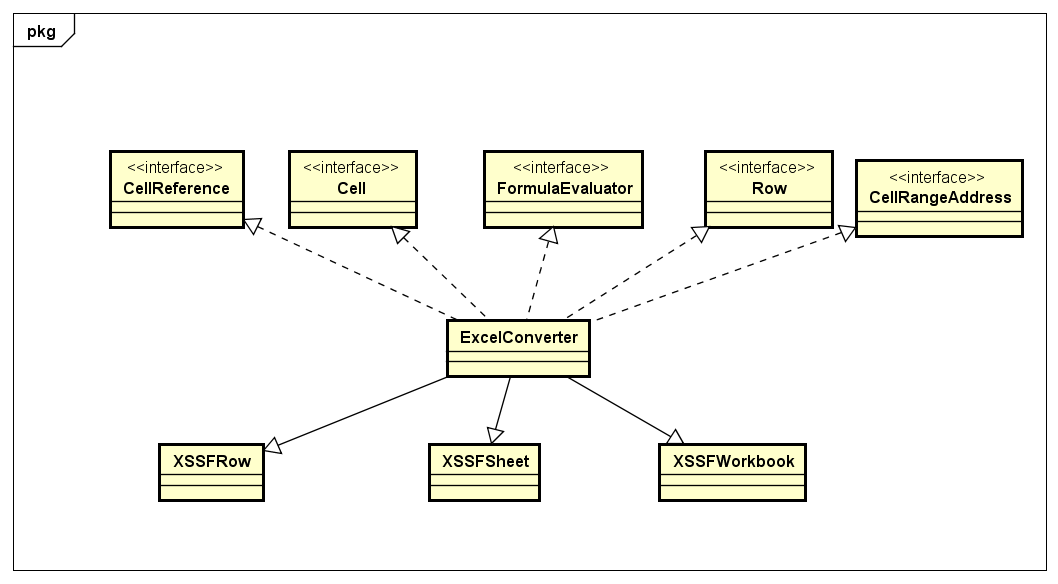
\includegraphics[scale=0.5]{Gambar/pemodelanExcelConverter}
	\caption{Gambar Pemodelan ExcelConverter}
	\label{fig:pemodelanExcelConverter}
\end{figure}

\begin{figure}[H]
	\centering
	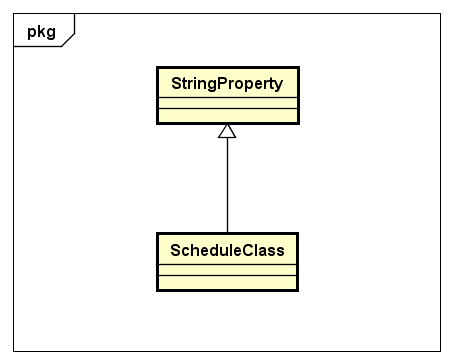
\includegraphics[scale=0.6]{Gambar/pemodelanScheduleClass}
	\caption{Gambar Pemodelan ScheduleClass}
	\label{fig:pemodelanExcelConverter}
\end{figure}
\begin{figure}[H]
	\centering
	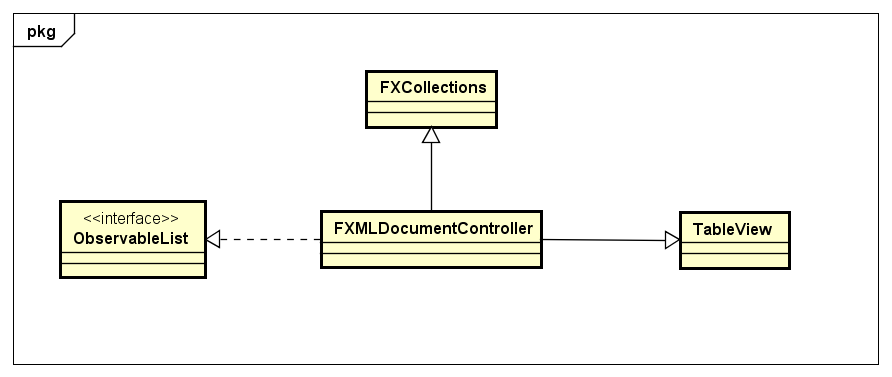
\includegraphics[scale=0.5]{Gambar/pemodelanFXMLDocumentController}
	\caption{Gambar Pemodelan FXMLDocumentController}
	\label{fig:pemodelanFXMLDocumentController}
\end{figure}


\begin{figure}[H]
	\centering
	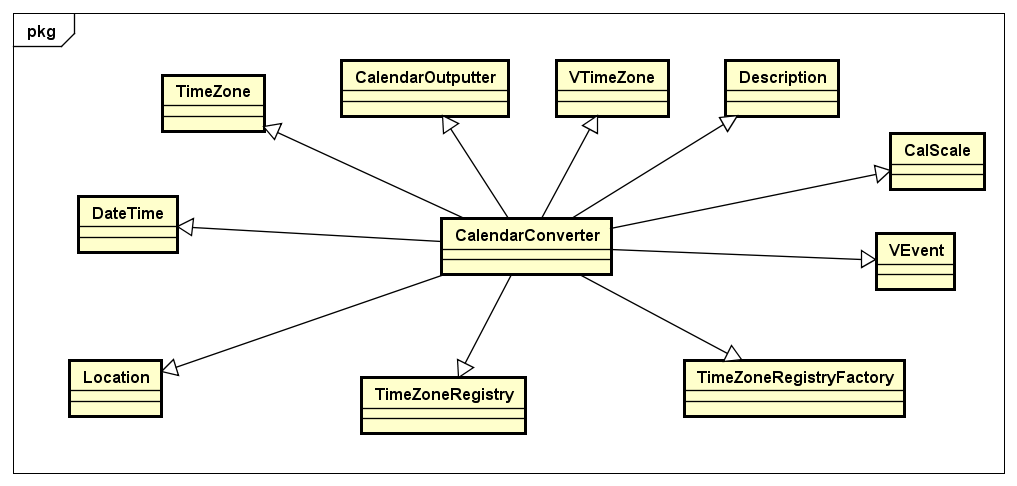
\includegraphics[scale=0.5]{Gambar/pemodelanCalendarConverter}
	\caption{Gambar Pemodelan CalendarConverter}
	\label{fig:pemodelanExcelConverter}
\end{figure}

\begin{figure}[H]
	\centering
	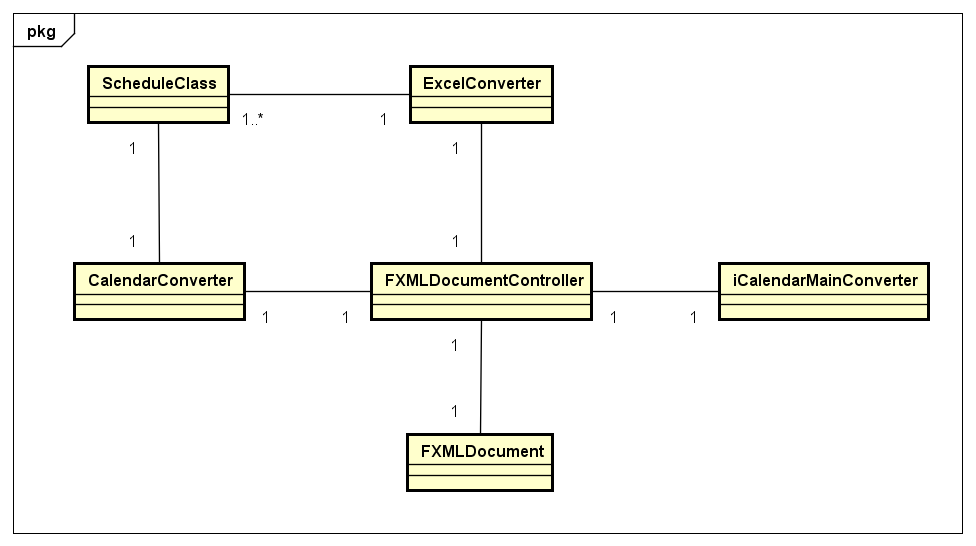
\includegraphics[scale=0.5]{Gambar/pemodelan-kelas}
	\caption{Gambar Pemodelan Kelas}
	\label{fig:pemodelanKelasSeluruh}
\end{figure}

Berikut penjelasan fungsi dari kelas dari gambar \ref{fig:pemodelanKelasSeluruh} :	
\begin{enumerate}
	\item \textbf{ScheduleClass}\\
	Kelas ini berfungsi menampung jadwal pengawas yang telah dikonversi oleh kelas ExcelConverter.
	\item \textbf{ExcelConverter}\\
	Kelas ini bertugas membaca file excel jadwal mengawas ujian sehingga dapat ditampilkan oleh perangkat lunak.
	\item \textbf{FXMLDocumentController}\\
	Kelas ini mempunyai peran untuk mendapatkan file \textit{input} yang dimasukkan oleh pengguna,  memberi perintah 
	kepada kelas ExcelConverter untuk membaca \textit{input}, menampilkannya kembali ke perangkat lunak dan memberikan perintah
	kepada CalendarConverter untuk mengkonversikannya dalam iCal.
	\item \textbf{CalendarConverter}\\
	Kelas ini berfungsi mengkonversi file yang telah dibaca kedalam format .ics atau iCalendar.
	\item \textbf{iCalendarMainConverter}\\
	kelas ini berfungsi sebagai \textit{main} pada perangkat lunak dimana kelas ini mengeksekusi dan menghubungkan seluruh elemen kelas 
	pada perangkat lunak ini.
\end{enumerate}
